\documentclass[12pt, oneside, a4paper]{report}

\usepackage{afterpage}   \usepackage{amsmath}     \usepackage{amssymb}
\usepackage{cancel}      \usepackage{enumitem}    \usepackage[english]{babel}
\usepackage{bold-extra}  \usepackage{booktabs}    \usepackage{caption}
\usepackage{cite}        \usepackage{fancyhdr}    \usepackage[T1]{fontenc}
\usepackage{geometry}    \usepackage{graphicx}

\usepackage[breaklinks, colorlinks=true, linkcolor=blue, linkcolor=blue,
    anchorcolor=blue, citecolor=blue, filecolor=blue, menucolor=blue,
    runcolor=blue, urlcolor=blue]{hyperref}

\usepackage{layout}      \usepackage{listings}    \usepackage{lscape}
\usepackage{makecell}    \usepackage{mathastext}  \usepackage[version=4]{mhchem}
\usepackage{multicol}    \usepackage{numprint}    \usepackage{setspace}
\usepackage{tikz}        \usepackage{times}       \usepackage{titlesec}
\usepackage{xcolor}      \usepackage{xurl}

\usetikzlibrary{calc}

% URL font
\urlstyle{same}

% \usepackage{showframe}

% Taille du tableau -0.5 cm
% \textheight = 731 pt
% \textwidth = 483 pt

\lstset{
    basicstyle=\footnotesize\ttfamily,
    emphstyle={\bfseries},
    escapeinside={(*}{*)},
    numbers=left,
    numberstyle=\scriptsize\color{black},
    tabsize=4,
    columns=fixed,
    frame=tb,
    showstringspaces=false,
    showtabs=false,
    keepspaces,
    emph={
        SI,
        SINON,
        RETOURNER,
        FIN,
        POUR,
        ALORS,
        \backslash\backslash,
        VARIABLE,
        INITIALISATION,
        TRAITEMENT,
        SORTIE
    },
    literate={à}{{\`a}}1
    {é}{{\'e}}1
    {è}{{\`e}}1
    {<-}{{$\leftarrow$}}1
}

\geometry{top = 2.5cm, bottom = 3.5cm, hmargin = 2.5cm}

\newcommand{\emptypage}{
    \newpage
    \null
    \thispagestyle{empty}
    \addtocounter{page}{-2}
    \newpage
}
\newcommand{\fref}[1]{\hyperref[#1]{\textbf{[fig.~\ref*{#1}]}}}
\newcommand{\subfref}[2]{\hyperref[#1]{\textbf{[fig.~\ref*{#1}~: #2]}}}
\newcommand{\tref}[1]{\hyperref[#1]{\textbf{[tab.~\ref*{#1}]}}}
\newcommand{\aref}[1]{\hyperref[#1]{\textbf{[\ref*{#1}]}}}
\newcommand{\saref}[1]{\hyperref[#1]{\textbf{[app.~\ref*{#1}]}}}
\newcommand{\eref}[1]{\textbf{[éq.~\eqref{#1}]}}
\newcommand{\eqdes}[1]{
    \begin{footnotesize}
        \hrule height 1pt
        #1
    \end{footnotesize}
}
\newcommand{\p}[1]{$^\text{#1}$}
\newcommand{\id}[1]{$_\text{#1}$}
\newcommand{\can}[1]{$\cancel{\text{#1}}$}
\newcommand{\mathBF}[1]{\mathbf{\boldsymbol{#1}}}
\newcommand{\ms}{\\[2em]}
\newcommand{\C}{\tiny$\blacksquare$}
\newcommand{\Cite}[1]{\p{\textbf{\cite{#1}}}}

\renewcommand{\theequation}{\thechapter{}.\arabic{equation}}
\renewcommand{\headrulewidth}{0pt}
\renewcommand{\thesection}{\arabic{section}}

\newenvironment{matheq}{
    \begin{equation*}
        \begin{array}{rcl}
}{
        \end{array}
    \end{equation*}
}
\newenvironment{f}{
    \begin{figure*}
        \begin{minipage}[c][\textheight][c]{\textwidth}
}{
        \end{minipage}
    \end{center}
}
\newcounter{exempleNumber}\setcounter{exempleNumber}{1}
\newenvironment{exemple}{
    \begin{itshape}
        \vspace{.5em}\footnotesize
        \phantom{M}\hfill\textbf{EXEMPLE~\arabic{exempleNumber}}\hfill\phantom{M}
        \vspace{.5em}
        
        \hrule\vspace{3pt}
}{
        \vspace{3pt}\hrule
    \end{itshape}\stepcounter{exempleNumber}
}
\makeatletter
\renewcommand\tableofcontents{%
    \@starttoc{toc}%
}
\renewcommand\listoffigures{%
        \@starttoc{lof}%
}
\renewcommand\listoftables{%
        \@starttoc{lot}%
}
\def\tagform@#1{\maketag@@@{\bfseries(\ignorespaces#1\unskip\@@italiccorr)}}
\makeatother
\setcounter{tocdepth}{3}
\setcounter{secnumdepth}{3}
\setlength{\parindent}{0pt}
\setlength{\parskip}{0.20cm}
\setlength{\headheight}{0pt}
\setlength{\columnsep}{2cm}
\titleformat{\section}[hang]
{\bfseries}
{\thesection.}
{1ex}
{}
\titleformat{\subsection}[hang]
{\bfseries}
{\thesubsection.}
{1ex}
{}
\titleformat{\subsubsection}[hang]
{}
{\phantom{\bfseries\thesubsection\hspace{1ex}}\thesubsubsection.}
{1ex}
{}
\captionsetup[figure]{font=footnotesize, labelfont=bf, name={Fig.}, labelformat=simple}
\captionsetup[table]{font=footnotesize, labelfont=bf, name={Tab.}, labelformat=simple}
\pagestyle{fancy}
\fancyhead[]{}
\fancyfoot[C]{--~\thepage{}~--}
\fancypagestyle{plain}{\fancyhf{}\fancyfoot[C]{--~\thepage{}~--}}

\title{Phylogeny report}
\author{Alexis BEL, Lucas ROUAUD}
\date{\today}
\begin{document}
\pagenumbering{arabic}
\begin{huge}
    \begin{flushleft}
        \textbf{KAGGLE PROJECT -- OpenVaccine:} COVID-19 mRNA vaccine degradation prediction
    
        \vspace{1ex}
        
        \hrule height 2pt
    \end{flushleft}
\end{huge}
\vspace{2ex}
\textit{\textbf{\large Document made with \LaTeX{}}}

\textbf{REPORTER:} Ms. GALOCHKINA T., M\p{r} GELLY J-C. and M\p{r} GUYON F.

\textbf{BEL Alexis, BELAKTIB Anas, OUSSAREN Mohamed, ROUAUD Lucas}

\textbf{Master 2 BI}: Université Paris Cité

\vspace{2ex}

\begin{center}
    \begin{minipage}{16cm}
        \hrule height 0.5pt width 16cm
        
        \vspace{2ex}
        
        \section*{Abstract}
        \paragraph*{Background}
        Kaggle is a worldwide competition of machine learning, where scientist are attempting to answer to a complex question. Here, the problem is on the prediction of the stability of mRNA for COVID-19 vaccine. Here, we tried to answer this question by using three different embedding on two different neural networks with the aim to compare these different methods.

        \vspace{2ex}
        
        \paragraph*{Results}
        We test two simple neural networks, which gave approximately the same results. The only differences is that the Google inception module converge quickly than the CNN one. In addition, the different input embedding give various results.
        
        \vspace{2ex}
        
        \paragraph*{Dispobility}
        The program, with the original dataset, are available at this Github page: \url{https://github.com/FilouPlains/KAGGLE_OPENVACCINE_MRNA}. 

        \vspace{2ex}
        
        \hrule height 0.5pt width 16cm
        
        \vspace{2ex}
        
        \begin{footnotesize}
            \bfseries ABBREVIATIONS: \textit{mRNA~=} messenger ribonucleic acid; \textit{CNN~=} convolutional neural network.
        \end{footnotesize}
    \end{minipage}
\end{center}

\vspace{2ex}

\begin{multicols}{2}
\section{Introduction}
\subsection{Context}
The COVID-19 is a mondial scale epidemics who paralyzed world's economics for almost 2 years\Cite{ciottiCOVID19Pandemic2020, bartikImpactCOVID19Small2020, longCOVID19PandemicIts2022}. To treat this disease, a quick vaccine has to be done. This is where mRNA vaccine are involved. They are quick to design and permits to immunize against a given a patient.

\begin{table*}[tb]
    \centering
    \begin{minipage}{10.86cm}
        \caption{\textbf{Lifespan of RNA vaccines at different temperature\Cite{crommelinAddressingColdReality2021b}.  
            \label{t:manufacturerFrozenRoomtemp} \vspace{-1em}}}
    \end{minipage}

    \begin{tabular}{llrlc}
        \toprule
        \bfseries Manufacturer  & \bfseries \phantom{$\sim$}Frozen State        & \multicolumn{2}{c}{\bfseries 2 -- 8~$^{\circ}$C}  &  \bfseries Room temperature\\
        \midrule
        Moderna                 & \phantom{$\sim$}6 months (-20~$^{\circ}$C)    & 30 & days                       & 12~h\\
        Pfizer                  & \phantom{$\sim$}6 months (-80~$^{\circ}$C)    & 5  & days                        & \phantom{0}2~h\\
        CureVac                 & $\sim$3 months (-60~$^{\circ}$C)              & 3  & months                      & 24~h\\
        \bottomrule
    \end{tabular}
\end{table*}

However, even if the mRNA vaccines are the fastest vaccine candidates for COVID-19, they still have a major issue: their lack of stability. Researchers have observed that RNA molecules tend to spontaneously degrade. Vaccine with degraded mRNA become deprecated to the population's vaccination\Cite{leppekCombinatorialOptimizationMRNA2022, verbekeThreeDecadesMessenger2019}. Currently, little is known on the details of where in the backbone of a given RNA is most prone to being affected. Without this knowledge, current vaccines against COVID-19 must be prepared and shipped under intense refrigeration, and are unlikely to reach more than a tiny fraction of human beings on the planet unless they can be stabilized. The \tref{t:manufacturerFrozenRoomtemp} contains the lifespan of different RNA vaccines against COVID-19. Each vaccine as a different temperature of conservation (frozen state) before they are use. When they are defrozen they must be immediately use before the vaccine start to degrade. The vaccination of the population must be organized to ensure that the vaccines are use efficiently for the two injections. 

This project, from a Kaggle competition sponsor by Das Lab at Stanford Biochemistry, aims to use machine learning to a have better understanding of the regions which are most likely to be degraded by using the local characteristic of the sequence. The competition finish in 2020 and an article was published on it\Cite{muneerIVaccineDeepPredictionCOVID192022}. To do that, the degradation rates at various locations along RNA sequence is predicted. Two major problems are notable. The first one is the various input size of the sequences. Indeed, they are either size of 107 or 130. The second one is the various output size, which will be  either 68 or 91 (depending on the input size sequence). In order to deal with these problems, mask are going to be design.

\subsection{Data}
Two datasets are available at Kaggle website: the first one contains 2,400 mRNA of 107 bases described by three descriptive variables that originate from Eterna\Cite{leeRNADesignRules2014}. These descriptive variables correspond to the RNA sequence, the structure and the predicted loop types assigned by bpRNA from Vienna RNAfold 2 structure. These variables describe the degradation rate in five values :

\begin{description}
    \item[reactivity:] These numbers are reactivity value and used to determine the likely secondary structure of the RNA sample.
    \item[deg\_pH10:] These numbers are reactivity value and used to determine the likelihood of degradation at the base/linkage after incubating without magnesium at pH 10.
    \item[deg\_Mg\_pH10:] These numbers are reactivity value and used to determine the likelihood of degradation at the base/linkage after incubating with magnesium at  pH 10.
    \item[deg\_50C:] These numbers are reactivity value and used to determine the likelihood of degradation at the base/linkage after incubating without magnesium at  50~$^{\circ}$C.
    \item[deg\_Mg\_50C:] These numbers are reactivity value and used to determine the likelihood of degradation at the base/linkage after incubating with magnesium at  50~$^{\circ}$C.
\end{description}

The second one contains 3,634 molecules among which there are 629 sequences of size 107 and 3,005 of size 130 were synthesized and characterized at the Stanford University.

\begin{figure*}[!tb]
    \centering
    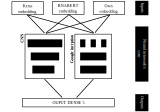
\includegraphics[width=\textwidth]{figure/Scheme_neural_network.pdf}
        
    \small
    \vspace{0.5ex}
    
    \hrule height 1pt
    
    \vspace{1ex}
    
    \caption{
        \textbf{Diagram of the neural network created for this Kaggle project.} It's divided in three part: the inputs, which are embedding with dimensionnal adjusment; the neural network's core, consisting of two differents modules; the ouputs. All combinaison (6 in total) have been tested.
        \label{f:Scheme_neural_network}}
\end{figure*}

\section{Materials and Methods}
To answer to the problematics, we decide to design a program which transform the input into three type of embedding and two module for the ``core'' \fref{f:Scheme_neural_network}.

\subsection{Program implementation}
The program was implemented in \texttt{python 3.10.6} using the module \texttt{keras 2.7.0} and \texttt{tensorflow 2.7.0}. The module \texttt{numpy 1.23.3} was also used to perform vectorial calculation.

\subsection{Hot encoding}
The one hot encoding consists in encoding the string sequences in vectors of different dimensions. Each string will be represented by a numpy array. The hot encoding is necessary before the embedding.

\subsection{Embedding}
Before feeding the data to the networks, we will use a three-way to embed the data. For two first methods, we used the sequences of RNA sequences, the sequences of the structure of RNA and the sequences of loop types of the RNA. For the third method, we only used the RNAs sequences.

\subsubsection{``Homade embedding''}
\begingroup
\centering
    \includegraphics[width=\columnwidth ]{figure/own_embedding.pdf}
        
    \small
    \vspace{0.5ex}
    
    \hrule height 1pt
    
    \vspace{1ex}
    
    \captionof{figure}{
        \textbf{Diagram showing how the ``homemade embedding'' are modified to be input into the neural network.} The convolution is 1D.
        \label{f:own_embedding}}
\endgroup

The first way of embedding was with our own methods. First, we hot encode the three sequences. The RNA sequence will give a sequence of vector of 4. The structure sequence will give a sequence of vector 3. The loop type sequence will give a sequence of vector 7.

Then we used a positional embedding by taking the odd position of the sequence and the pair position:
\begin{itemize}
    \item[\C] For the odd position, we use the formula:
\end{itemize}

\begin{matheq}
    E_{p(pos, ~2 \times i)} = \sin\left(\dfrac{pos}{1 \cdot 10,000^{\dfrac{2 \times i}{d}}} \right)
\end{matheq}
    
\begin{itemize}    
    \item[\C] For the pair position, we use the formula:
\end{itemize}

\begin{matheq}
    E_{p(pos, ~2 \times i + 1)} = \cos\left(\dfrac{pos}{1 \cdot 10,000^{\dfrac{2 \times i}{d}}} \right)
\end{matheq}

\paragraph{For the above equation} \textit{E\id{p}~=} positional embedding; \textit{pos~=} the index of the embedding or, here, the index of the sequence; \textit{i~=} the index of the positional embedding or, here, the index of the base. 
With these methods, three embedded sequences of vector 4, 3 and 7 were obtained \fref{f:own_embedding}.

\subsubsection{Keras embedding}
For the second way of embedding show in \fref{f:keras_embedding}, the function of the module Keras ``embedding'' was used. We hot encoded the three sequences, then we gave the sequences to the Keras embedding. The Keras embedding gave us three sequences of vectors.

\begingroup
\centering
    \includegraphics[width=\columnwidth ]{figure/keras_embedding.pdf}
        
    
    \hrule height 1pt
    

    \captionof{figure}{
        \textbf{Diagram showing the embedding by keras.} The convolution is 1D.
        \label{f:keras_embedding}}
\endgroup

\subsubsection{RNABERT embedding}
For the third way of embedding, we used come from the article ``Informative RNA base embedding for RNA structural alignment and clustering by deep representation''\Cite{akiyamaInformativeRNABase2022}.  We used the neural network that was pre-trained on the database Rfam 14.3. This neural network will embed the RNA sequence in sequences of vector of 120 values. This embedding encode the characteristics of each RNA family and structures. 

We give an RNA sequences to the network that will generate a 120 vector that encode for A, C, G and T for each base. Then the position embedding will generate a vector of 120 that encode the position of each base. Finally, the two vector is sum and given to the transformer. The transformer will return a sequence of length l of vector 120 that is informative base.

\vspace{-2ex}

\subsection{Neural network}
During the study, we use two neural network modules: a convolutional neural network and an inception module.

\vspace{-2ex}

\subsubsection{CNN}
The first deep learning approach was a convolutional neural network (CNN). This CNN has 4 layers with a kernel initializer: he\_uniform, and an activation: Relu with a 0,2 dropout. The model was then compiled using the Adam optimizer \fref{f:cnn}. 
\begin{matheq}

    MCRMSE & = & \dfrac{1}{m} \times \displaystyle\sum^m_{j = 1} RMSE_j \ms
 
    RMSE_j & = & \sqrt{\dfrac{\displaystyle\sum^n_{i = 1}\left(y_{ij} - \hat{y}_{ij}\right)^2}{n}}
\end{matheq}

\paragraph{For the above equation} \textit{MCRMSE~=} Mean Column-wise Root Mean Squared Error; \textit{m~=} number of predicted variables; \textit{n~=} number of test samples; \textit{y\id{ij}~=} i\p{th} actual/real value of j\p{th} variable; \textit{$\hat{y}_{ij}$~=} i\p{th} predicted value of j\p{th} variable.

\begingroup
\centering
    \includegraphics[width=\columnwidth ]{figure/cnn.pdf}
        
    
    \hrule height 1pt
    

    \captionof{figure}{
        \textbf{Diagram showing the model CNN.} The convolution is 1D.
        \label{f:cnn}}
\endgroup

\begin{figure*}[!tb]
    \centering
    \includegraphics[width=\textwidth]{figure/inception.pdf}
        
    \small
    \vspace{0.5ex}
    
    \hrule height 1pt
    
    \vspace{1ex}
    
    \caption{
        \textbf{Diagram showing the model inception.} The convolution and the maxpooling are 1D.
        \label{f:inception}}
\end{figure*}

\subsection{Inception}
The second deep learning approach was an inception model\Cite{szegedyGoingDeeperConvolutions2014}. This model is divided into two parts \fref{f:inception}. The first part  is a set of convolutional layers with a dropout that will be concataned and injected in the second part. The second part is composed of dense layers of decreasing filters size. The model was then compiled using the Adam optimizer.


\subsubsection{Non Cross-validation}
To establish the best model, the number of epoch was established at 500 and the batch size at 50. The training data was divided by 20~\% to estimate the fitting of the model.
The best model was selected by looking at the validation loss between each epoch. When this loss decreases the model was safe, but if the loss didn't show any change for 10 epochs by a value of 0.001 the fitting is stopped.

\begin{figure*}[!tb]
    \centering
    \includegraphics[width=\textwidth]{figure/loss_function.pdf}
        
    \small
    \vspace{0.5ex}
    
    \hrule height 1pt
    
    \vspace{1ex}
    
    \caption{
        \textbf{Plot of the different tested neural network.} \textit{KE~=} Keras' embedding; \textit{RB~=} RNABERT's embedding; \textit{HM~=} ``homemade'' embedding; \textit{L~=} loss evolution; \textit{VL~=} validation losss evolution. Some curve does not do all Epochs, as far as the program keep only the best model.
        \label{f:loss_function}}
\end{figure*}

\section{Result}
The first experiment was to build a pre-CNN to perform pre-processing on the given inputs. The three types of data are not structured in the same way. From this data, we define 2 neural networks of different architecture. This CNN will be compared in order to evaluate their performance. The proposed approach has been evaluated on a remote Cluster server having the characteristics of being hyperthreaded (numerous cores) to decrease the execution time.

\subsection{CNN}
Preliminary results from the CNN help to show the effectiveness and predictive ability. The results below were performed on the training datasets.

According to the figure \fref{f:loss_function}, the three fitted models have different epochs: the model keras stopped at the epoch 154; the model own at the epochs 59 and the model re at the epoch 137.

 Globally, the CNN shows good performances according to the provided embedding types. Indeed, as illustrated on the figure above, the model keras and the model own seems to have similar values of loss but with a different number of epochs. The model owe obtain the values faster than the model keras.
The models re has the lower values of loss and validation loss than the others. The model seems the most efficient. We can also remark that the model has a better capacity of generalization, with values of loss and validation loss close.

\begin{table*}[!tb]
    \centering
    \begin{minipage}{9.92cm}
        \caption{\textbf{Result publish on Kaggle\Cite{muneerIVaccineDeepPredictionCOVID192022}. The random result come from a submission containing random number.  
            \label{t:result_kaggle} \vspace{-1em}}}
    \end{minipage}

    \begin{tabular}{lcc}
        \toprule
        \bfseries Model             & \bfseries Public score        & \bfseries Private score\\
        \midrule
        Best model from KAGGLE      & 0.22614                       & 0.34152\\
        This paper best model       & 0.51887                       & 0.58209\\
        Random                      & 0.58349                       & 0.64742\\
        \bottomrule
    \end{tabular}
\end{table*}

\subsection{Inception}
By applying a neuronal network following the model of Google Inception slightly modified, we have three fitted models with differents epochs: the model keras stopped at the epoch 101; the model own at the epochs 65 and the model re at the epoch 58.


The figure \fref{f:loss_function} represent the loss and the validation loss of the three models. The model own seems to be the most over-fitted. The keras model has his values of loss and validation parallel that indicates a good fitting.
The best model is yet again the model re with the lowest value of loss and validation loss and with the smaller difference between the two values. This model is the most efficient and the most generalize.

\subsection{The optimal neuronal network} 
By comparing the loss and the validation loss of the 6 models, the best model can be estimated. The criteria of selection are the generalization (over or under fitting) and the value of loss. As we can see, the curve of the model RNABERT are close in value and shape, indicating a better generalization than the others. Also, it has the lowest value of loss and validation loss. The result of the model give better result that a model tha a random model \tref{t:result_kaggle}.

\section*{Conclusion}
For the three models, we can see that the different way of embedding have an effect on the prediction. The most efficient model is the one with the embedding from RNABERT on the model inception.

\section*{References}
\begingroup
    \begin{footnotesize}
        \renewcommand{\chapter}[2]{}%
        % List of style here : /usr/share/texlive/texmf-dist/bibtex/bst
        \bibliographystyle{naturemag}
        \bibliography{IEEEabrv, references.bib}
    \end{footnotesize}
\endgroup
\end{multicols}
\end{document}  